\chapter{Metodologia de desenvolvimento}

Para a realização deste trabalho, foi planejada uma metodologia de desenvolvimento na qual objetivou-se a construção da arquitetura do SMA por meio de uma metologia de desenvolvimento de SMAs. Inicialmente, foi necessário um levantamento de bibliografias relacionadas à Informática na Educação para o entendimento do problema do trabalho, além de levantamentos de uso de SMA em contextos pegagógicos.

Em seguida foi aplicada, foi realizado estudos aprofundados na metodologia MASE para a implementação deste trabalho. Após o levantamento inicial, seu uso é divido em duas fases, conforme explicado na seção~\ref{section:mase}, sendo a primeira delas essêncial para o levantamento dos requisitos necessários para cumprir os objetivos. A segunda fase foi importante para a distribuição das regras entre os agentes que existem no sistema. As primeiras subseções deverão detalhar a modelagem.

A arquitetura do sistema já havia sido previamente decidida~\cite{editalFrank}, sendo necessário adequar os requisitos do trabalho à arquitetura proposta por meio da metodologia MASE. Neste mesmo documento, foi definido o nome da solução à ser desenvolvida:~\emph{Frank}.

Posteriormente o trabalho seguiu-se com a implementação do SMA na linguagem JAVA, utilizando-se das ferramentas JADE e JBoss Seam. As subseções seguintes deverão detalhar a implementação do Sistema Multiagente e da camada web, bem como a sua integração.

Por fim, a solução foi testada por meio de cenários que simulavam o uso por meio dos atores Aluno e Docente. A demonstração está detalhada no capítulo 4.

\section{A Modelagem}

A modelagem foi desenvolvida utilizando-se a ferramenta~\emph{agentTool}. A ferramenta possui meios para diagramar todas as fases e passos do MASE, auxiliando o analista em todos os diagramas necessários, além de gerar código automático para alguns frameworks de SMA.

Conforme dito a respeito do MASE, a metodologia é dividida em duas fases: Análise e Design. A primeira fase, responsável pelo levantamento de requisitos e entendimento das regras e tarefas, é apresentada na subseção~\ref{subsection:analise}. A segunda fase está apresentada em~\ref{subsection:design}.

\subsection{Análise}\label{subsection:analise}

A metodologia inicia-se com o passo de captura das metas. Para tanto, foi necessário primeiramente um levantamento inicial dos requisitos do SMA. Os requisitos foram levantados e compreendidos por meio de~\cite{editalFrank}, onde é possível listar:

\begin{enumerate}
	\item O sistema deve manter um modelo do estudante, onde será determinado o seu estilo de aprendizagem e será notíficado ao docente.
	\item O sistema deve assistir (auxiliar) o aluno por meio de um grupo de trabalho.
	\item O sistema deve fazer interface com Ambiente Virtual de Aprendizagem, a fim de estabelecer comportamentos do estudante.
	\item O sistema deve criar uma modelagem cognitiva do aluno, onde são mantidas informações sobre o desempenho, de acordo sua interação em Ambiente Virtual de Aprendizagem, e informações a respeito do seu estilo de aprendizagem.
	\item O sistema deve criar uma modelagem metacognitiva do aluno, onde são armazenadas informações com o intuito de melhorar processos de aprendizagem de domínios específicos.
	\item O sistema deve criar uma modelagem afetiva do estudante, especificamente a respeito da modelagem da personalidade e emoções do estudante.
	\item O sistema deve fazer interface com Ambiente Virtual de Aprendizagem.
	\item O sistema deve refutar ou confirmar o estilo de aprendizagem do aluno a partir do desempenho relacionado à interação com o sistema e/ou com Ambiente Virtual de Aprendizagem.
	\item O sistema SMA deve atualizar o modelo do estudante com base em inferências a partir dos registros de trabalho do estudante.
	\item O sistema deve construir o modelo do estudante a partir de uma modelagem explícita, ou seja, a partir do feedback explícito do estudante (questionário).
	\item O sistema deve construir o modelo do estudante a partir de uma modelagem implícita, ou seja, a partir do desempenho obtido nas ferramentas de aprendizado.
\end{enumerate}

A partir dos requisitos de~\cite{editalFrank}, foi possível estabelecer metas que o sistema deveria atingir para satisfazê-los:

\begin{itemize}
	\item Manter um modelo do estudante (Meta geral do sistema)
	\item Notificar ao docente
	\item Auxiliar o aluno por meio de um grupo de trabalho
	\item Criar modelagem cognitiva
	\item Criar modelagem metacognitiva
	\item Criar modelagem modelagem afetiva
	\item Criar modelagem da personalidade
	\item Criar modelagem das emoções do estudante
	\item Interface com ferramentas de aprendizagem dedicada
	\item Confirmar estilo de aprendizagem do aluno
	\item Refutar estilo de aprendizagem do aluno
	\item Construir modelo de desempenho do aluno
	\item Construir modelagem explícita
	\item Construir modelagem implícita
	\item Construir modelo de estilo de aprendizagem do aluno
\end{itemize}

A partir do levantamento, foi possível observar que a meta "Manter um modelo do estudante" abrange o escopo geral de toda a aplicação, sendo possível estabelecer como meta do sistema. Em seguida, foi necessário hierarquizar as metas de forma a encontrar quais metas poderiam ser estabelecidas com o cumprimento de outras. A imagem~\ref{fig:metas-frank} representa a hierarquia de metas que foi estabelecida. Os retângulos em cinza representam metas particionadas.

\begin{sidewaystable}
	\centering
	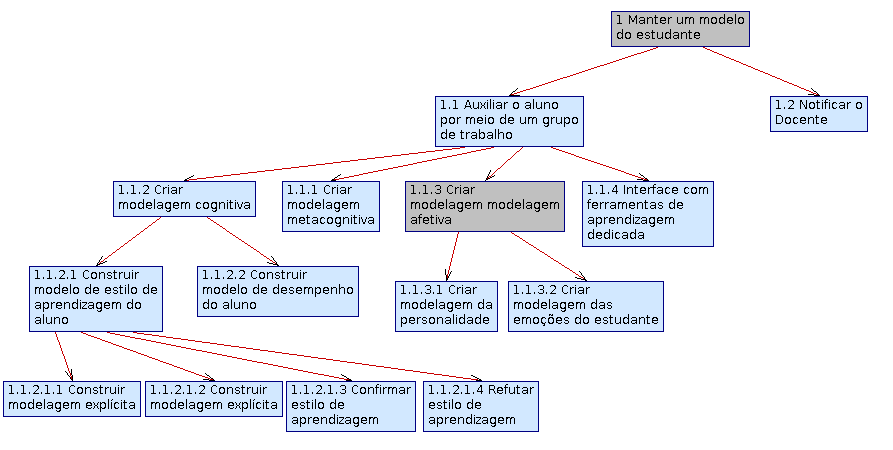
\includegraphics[scale=0.8]{images/metas-frank.png}
	\caption{Hierarquia de Metas do SMA Frank.}
	\label{fig:metas-frank}
\end{sidewaystable}

O segundo passo da metodologia consiste no desenvolvimento dos casos de uso. Foram levantados 5 principais casos de uso, alguns com fluxos alternativos que representam situações opcionais no caso de uso. Este trabalho utiliza-se da notação completa de desenvolvimento de casos de uso.

O primeiro caso de uso descreve o cenário de notificação do docente. Nele, o docente é autenticado no sistema e o sistema exibe uma lista de alunos disponíveis nas mais diversas turmas. O docente seleciona um aluno e então o sistema exibe os dados relativos ao modelo do aluno. O trecho~\ref{code:uc-notificar-docente} possui a descrição do caso de uso.

\begin{usecase}

\addtitle{Caso de Uso 1}{Determinar Modelagem Cognitiva do Aluno}

\addfield{Escopo:}{Sistema e Ambiente(s) Virtuais(ns) de Aprendizagem(s)}
\addfield{Nível:}{Objetivo do sistema}
\addfield{Ator Principal:}{Sistema}

\additemizedfield{Interessados e Interesses:}{
	\item Sistema: Manter um modelo do estilo de aprendizagem do estudante a partir dos dados gerados do formulário, bem como com algum Ambiente Virtual de Aprendizagem.
	\item Aluno: Preencher o questionário de estilos de aprendizagem e interagir com um Ambiente Virtual de Aprendizagem.
}

\addfield{Pré-condições:}{Não se aplica}
\addfield{Pós-condições:}{}

\addscenario{Cenário de Sucesso Principal:}{
	\item O Aluno faz o primeiro login no sistema.
	\item O Sistema reconhece o perfil do aluno e cria um Grupo de Trabalho (GT) de agentes.
	\item O Aluno deverá preencher o questionário de estilos de aprendizagem.
	\item O Sistema avalia as respostas preenchidas pelo aluno e, conforme a literatura de psicologia, determinará o estilo de aprendizagem por meio da avaliação explícita.
	\item O Sistema construirá o primeiro modelo do aluno, com base no seu estilo de aprendizagem inicial.
	\item O Sistema salva os dados, a fim de notificar o docente dos dados obtidos.
	\item O Sistema notifica o Aluno sobre o seu estilo de aprendizagem.
	\item O Sistema exibe a lista de Ambiente Virtual de Aprendizagem disponíveis para o Aluno.
}

\addscenario{Extensões:}{
	\item[1.a] Falha no login:
		\begin{enumerate}
		\item[1.] O Sistema mostra mensagem de falha.
		\item[2.] O Docente retorna ao passo 1.
		\end{enumerate}
	\item[2.a] Inferência implícita de estilo de aprendizagem:
		\begin{enumerate}
		\item[1.] O Aluno faz login no sistema
		\item[2.] O Sistema reconhece o perfil do aluno e cria um grupo de trabalho de agentes.
		\item[3.] O Sistema exibe a lista de Ambiente Virtual de Aprendizagem (AVA) disponíveis para o Aluno.
		\item[4.] O Aluno seleciona o AVA
		\item[5.] O Sistema é notificado do AVA escolhido
		\item[6.] O AVA registra as ações do Aluno e envia para o Sistema.
		\item[7.] O AVA interage com o Sistema por meio do caso de uso.
		\item[8.] O Sistema utiliza os resultados de atividades feitas pelo aluno para inferir o seu estilo de aprendizagem, levando em consideração a literatura da psicologia relativa à atividade desenvolvida.
		\item[9.] O Sistema compara então os dados obtidos com os dados previamente armazenados, a fim de obter um grau de certeza do estilo de aprendizagem que foi construído.
		\item[10.] O Sistema salva os dados, a fim de notificar o Docente dos dados obtidos.
		\end{enumerate}
	\item[3.a] Inferência implícita de estilo de aprendizagem:
		\begin{enumerate}
		\item[1.] O Sistema analisa os dados obtidos do ambiente para determinar o desempenho do Aluno na atividade, levando em consideração a literatura pedagógica relativa.
		\item[2.] O Sistema salva os dados no banco de dados, a fim de notificar o Docente dos dados obtidos.
		\end{enumerate}
}

\addscenario{Requisitos Especiais:}{
	\item Não se aplica
}

\addscenario{Lista de Variantes Tecnologias de Dados:}{
	\item Não se aplica
}

\addfield{Frequência de Ocorrência:}{Sempre}

\end{usecase}
\label{code:uc-notificar-docente}


O segundo caso de uso diz respeito à modelagem cognitiva do aluno. Existem dois cenários possíveis: Modelagem implícita (principal cenário de sucesso) e modelagem explícita (cenário alternativo). Basicamente o SMA deverá processar o questionário respondido pelo aluno para inferir explicitamente o seu modelo cognitivo e deverá analisar as respostas enviadas por ele para inferir explicitamente o seu modelo cognitivo.



\begin{lstlisting}[label=code:uc-modelagem-cognitiva,caption=Caso de Uso - Notificar Docente.]
----------------------------------------------------
* UC 2 - DETERMINAÇÃO DA MODELAGEM COGNITIVA DO ALUNO
Escopo: Aplicação SMA e Ambiente(s) Virtual de Aprendizagem
Nível: Objetivo do sistema
Ator Principal: Sistema, Aluno
Interessados e Interesses:
	- Sistema: Manter um modelo do estilo de aprendizagem do estudante
a partir dos dados gerados da sua interação com um Ambiente Virtual
de Aprendizagem, bem como com o próprio sistema.
	- Aluno: Interagir com um ambiente de aprendizagem, bem como
a fim de obter parâmetros a respeito do seu modelo cognitivo.

Principal Cenário de Sucesso:
	1. O Aluno faz o primeiro login no sistema.
	2. O Sistema reconhece o perfil do aluno e cria um
Grupo de Trabalho (GT) de agentes.
	3. O Aluno deverá preencher um questionário onde seu
estilo de aprendizagem será deduzido por meio da avaliação explícita.
	4. O Sistema avalia as respostas preenchidas pelo aluno e,
conforme a literatura de psicologia, determinará o estilo de aprendizagem.
	5. O Sistema construirá o primeiro modelo do aluno, com base no
seu estilo de aprendizagem inicial.
	6. O Sistema salva os dados, a fim de notificar o docente dos
dados obtidos.
	7. O Sistema notifica o Aluno sobre o seu estilo de aprendizagem.
	8. O Sistema exibe a lista de Ambiente Virtual de
Aprendizagem disponíveis para o Aluno.

Extensões
	1 Inferência implícita de estilo de aprendizagem
		1.1. O Aluno faz login no sistema
		1.2. O Sistema reconhece o perfil do aluno e cria um grupo
de trabalho de agentes.
		1.3. O Sistema exibe a lista de Ambiente Virtual de
Aprendizagem disponíveis para o Aluno.
		1.4. O Aluno seleciona o AVA
		1.5. O Sistema é notificado do AVA escolhido
		1.6. O Ambiente Virtual de Aprendizagem registra as ações
do Aluno e envia para o Sistema.
		1.7. O ambiente interage com o Sistema por meio do caso de
uso UC5
		1.8. O Sistema utiliza os resultados de atividades feitas
pelo aluno para inferir o seu estilo de aprendizagem, levando em
consideração a literatura da psicologia relativa à atividade desenvolvida.
		1.9. O Sistema compara então os dados obtidos com os
dados previamente armazenados no banco de dados, a fim de obter um grau
de certeza do estilo de aprendizagem que foi construído. UC2.1
		1.9.1. O Sistema salva os dados no banco de dados, a fim de
notificar o Docente dos dados obtidos.

	2 Determinação do Desempenho do Aluno
		2.1. O Sistema analisa os dados obtidos do ambiente para
determinar o desempenho do Aluno na atividade, levando em consideração
a literatura pedagógica relativa.
		2.2. O Sistema salva os dados no banco de dados, a fim de
notificar o Docente dos dados obtidos.

Requisitos Especiais
	Não se aplica

\end{lstlisting}










\subsection{Design}\label{subsection:design}
